\documentclass{standalone}
\usepackage{tikz}
\usetikzlibrary{patterns, positioning}
\usepackage[sfdefault]{ClearSans} %% option 'sfdefault' activates Clear Sans as the default text font
\usepackage[T1]{fontenc}

\begin{document}
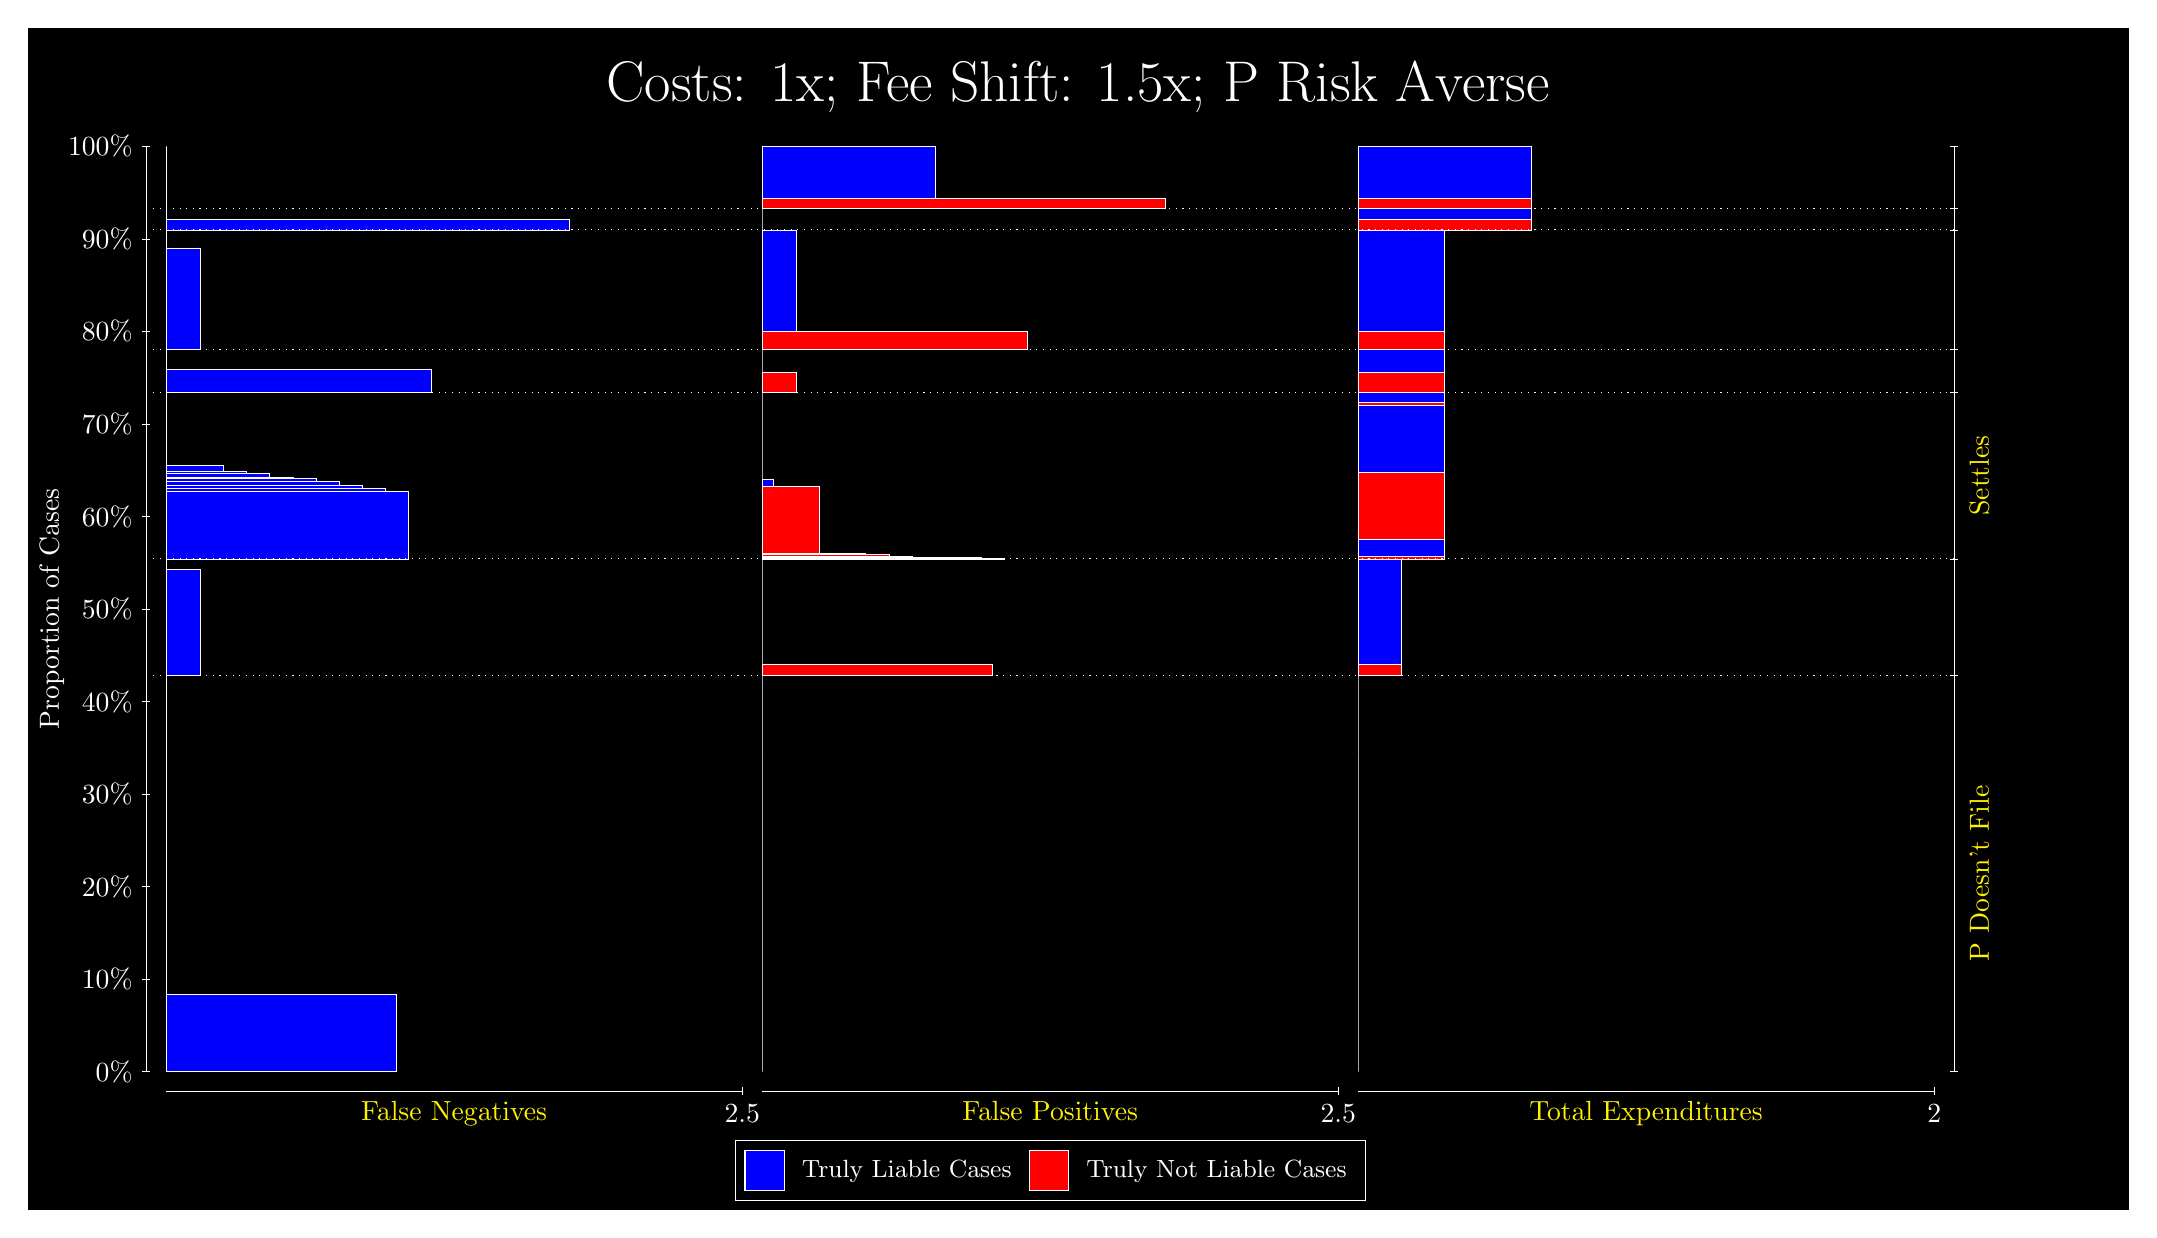
\begin{tikzpicture}
\draw[fill=black] (0,0) rectangle (26.667,15);
\draw[text=white] (0,13.5) rectangle (26.667,15) node[midway] {\huge Costs: 1x; Fee Shift: 1.5x; P Risk Averse};
\draw[white, very thin] (1.5,1.75) -- (1.5,13.5);
\node[rotate=90, text=white, anchor=center] at (0.3, 7.625) {Proportion of Cases};
\draw[white, very thin] (1.45,1.75) -- (1.55,1.75);
\node[text=white, anchor=east] at (1.45, 1.75) {0\%};
\draw[white, very thin] (1.45,2.925) -- (1.55,2.925);
\node[text=white, anchor=east] at (1.45, 2.925) {10\%};
\draw[white, very thin] (1.45,4.1) -- (1.55,4.1);
\node[text=white, anchor=east] at (1.45, 4.1) {20\%};
\draw[white, very thin] (1.45,5.275) -- (1.55,5.275);
\node[text=white, anchor=east] at (1.45, 5.275) {30\%};
\draw[white, very thin] (1.45,6.45) -- (1.55,6.45);
\node[text=white, anchor=east] at (1.45, 6.45) {40\%};
\draw[white, very thin] (1.45,7.625) -- (1.55,7.625);
\node[text=white, anchor=east] at (1.45, 7.625) {50\%};
\draw[white, very thin] (1.45,8.8) -- (1.55,8.8);
\node[text=white, anchor=east] at (1.45, 8.8) {60\%};
\draw[white, very thin] (1.45,9.975) -- (1.55,9.975);
\node[text=white, anchor=east] at (1.45, 9.975) {70\%};
\draw[white, very thin] (1.45,11.15) -- (1.55,11.15);
\node[text=white, anchor=east] at (1.45, 11.15) {80\%};
\draw[white, very thin] (1.45,12.325) -- (1.55,12.325);
\node[text=white, anchor=east] at (1.45, 12.325) {90\%};
\draw[white, very thin] (1.45,13.5) -- (1.55,13.5);
\node[text=white, anchor=east] at (1.45, 13.5) {100\%};

\draw[white, very thin] (24.457,1.75) -- (24.457,13.5);
\draw[white, very thin] (24.407,1.75) -- (24.507,1.75);
\node[anchor=west] at (24.407, 1.75) {};
\draw[white, very thin] (24.407,6.7835) -- (24.507,6.7835);
\node[anchor=west] at (24.407, 6.7835) {};
\draw[white, very thin] (24.407,8.2607) -- (24.507,8.2607);
\node[anchor=west] at (24.407, 8.2607) {};
\draw[white, very thin] (24.407,10.379) -- (24.507,10.379);
\node[anchor=west] at (24.407, 10.379) {};
\draw[white, very thin] (24.407,10.923) -- (24.507,10.923);
\node[anchor=west] at (24.407, 10.923) {};
\draw[white, very thin] (24.407,12.439) -- (24.507,12.439);
\node[anchor=west] at (24.407, 12.439) {};
\draw[white, very thin] (24.407,12.71) -- (24.507,12.71);
\node[anchor=west] at (24.407, 12.71) {};
\draw[white, very thin] (24.407,13.5) -- (24.507,13.5);
\node[anchor=west] at (24.407, 13.5) {};

\draw[white, very thin, fill=blue] (1.75,1.75) rectangle (4.6775,2.7317);
\draw[white, very thin, fill=red] (1.75,2.7317) rectangle (1.75,6.7835);
\draw[white, very thin, fill=blue] (1.75,6.7835) rectangle (2.1891,8.1251);
\draw[white, very thin, fill=red] (1.75,8.1251) rectangle (1.75,8.2607);
\draw[white, very thin, fill=blue] (1.75,8.2607) rectangle (4.8239,9.1209);
\draw[white, very thin, fill=blue] (1.75,9.1209) rectangle (4.5312,9.1541);
\draw[white, very thin, fill=blue] (1.75,9.1541) rectangle (4.2384,9.1899);
\draw[white, very thin, fill=blue] (1.75,9.1899) rectangle (3.9457,9.2467);
\draw[white, very thin, fill=blue] (1.75,9.2467) rectangle (3.6529,9.2878);
\draw[white, very thin, fill=blue] (1.75,9.2878) rectangle (3.3602,9.2957);
\draw[white, very thin, fill=blue] (1.75,9.2957) rectangle (3.0674,9.3432);
\draw[white, very thin, fill=blue] (1.75,9.3432) rectangle (2.7746,9.3693);
\draw[white, very thin, fill=blue] (1.75,9.3693) rectangle (2.4819,9.4537);
\draw[white, very thin, fill=red] (1.75,9.4537) rectangle (1.75,10.379);
\draw[white, very thin, fill=blue] (1.75,10.379) rectangle (5.1167,10.666);
\draw[white, very thin, fill=red] (1.75,10.666) rectangle (1.75,10.923);
\draw[white, very thin, fill=blue] (1.75,10.923) rectangle (2.1891,12.206);
\draw[white, very thin, fill=red] (1.75,12.206) rectangle (1.75,12.439);
\draw[white, very thin, fill=blue] (1.75,12.439) rectangle (6.8732,12.572);
\draw[white, very thin, fill=red] (1.75,12.572) rectangle (1.75,12.71);
\draw[white, very thin, fill=red] (1.75,12.71) rectangle (1.75,12.846);
\draw[white, very thin, fill=blue] (1.75,12.846) rectangle (1.75,13.5);
\draw[white, very thin, fill=red] (9.3189,1.75) rectangle (9.3189,5.8018);
\draw[white, very thin, fill=blue] (9.3189,5.8018) rectangle (9.3189,6.7835);
\draw[white, very thin, fill=red] (9.3189,6.7835) rectangle (12.246,6.9191);
\draw[white, very thin, fill=blue] (9.3189,6.9191) rectangle (9.3189,8.2607);
\draw[white, very thin, fill=red] (9.3189,8.2607) rectangle (12.393,8.2718);
\draw[white, very thin, fill=red] (9.3189,8.2718) rectangle (12.1,8.2756);
\draw[white, very thin, fill=red] (9.3189,8.2756) rectangle (11.807,8.2824);
\draw[white, very thin, fill=red] (9.3189,8.2824) rectangle (11.515,8.2843);
\draw[white, very thin, fill=red] (9.3189,8.2843) rectangle (11.222,8.2976);
\draw[white, very thin, fill=red] (9.3189,8.2976) rectangle (10.929,8.2981);
\draw[white, very thin, fill=red] (9.3189,8.2981) rectangle (10.929,8.3141);
\draw[white, very thin, fill=red] (9.3189,8.3141) rectangle (10.636,8.3256);
\draw[white, very thin, fill=red] (9.3189,8.3256) rectangle (10.344,8.3364);
\draw[white, very thin, fill=red] (9.3189,8.3364) rectangle (10.051,9.1858);
\draw[white, very thin, fill=blue] (9.3189,9.1858) rectangle (9.4652,9.2701);
\draw[white, very thin, fill=blue] (9.3189,9.2701) rectangle (9.3189,10.379);
\draw[white, very thin, fill=red] (9.3189,10.379) rectangle (9.758,10.635);
\draw[white, very thin, fill=blue] (9.3189,10.635) rectangle (9.3189,10.923);
\draw[white, very thin, fill=red] (9.3189,10.923) rectangle (12.686,11.156);
\draw[white, very thin, fill=blue] (9.3189,11.156) rectangle (9.758,12.439);
\draw[white, very thin, fill=red] (9.3189,12.439) rectangle (9.3189,12.577);
\draw[white, very thin, fill=blue] (9.3189,12.577) rectangle (9.3189,12.71);
\draw[white, very thin, fill=red] (9.3189,12.71) rectangle (14.442,12.846);
\draw[white, very thin, fill=blue] (9.3189,12.846) rectangle (11.515,13.5);
\draw[white, very thin, fill=red] (16.888,1.75) rectangle (16.888,5.8018);
\draw[white, very thin, fill=blue] (16.888,5.8018) rectangle (16.888,6.7835);
\draw[white, very thin, fill=red] (16.888,6.7835) rectangle (17.437,6.9191);
\draw[white, very thin, fill=blue] (16.888,6.9191) rectangle (17.437,8.2607);
\draw[white, very thin, fill=red] (16.888,8.2607) rectangle (17.986,8.2981);
\draw[white, very thin, fill=blue] (16.888,8.2981) rectangle (17.986,8.5073);
\draw[white, very thin, fill=red] (16.888,8.5073) rectangle (17.986,9.3567);
\draw[white, very thin, fill=blue] (16.888,9.3567) rectangle (17.986,10.217);
\draw[white, very thin, fill=red] (16.888,10.217) rectangle (17.986,10.255);
\draw[white, very thin, fill=blue] (16.888,10.255) rectangle (17.986,10.379);
\draw[white, very thin, fill=red] (16.888,10.379) rectangle (17.986,10.635);
\draw[white, very thin, fill=blue] (16.888,10.635) rectangle (17.986,10.923);
\draw[white, very thin, fill=red] (16.888,10.923) rectangle (17.986,11.156);
\draw[white, very thin, fill=blue] (16.888,11.156) rectangle (17.986,12.439);
\draw[white, very thin, fill=red] (16.888,12.439) rectangle (19.083,12.577);
\draw[white, very thin, fill=blue] (16.888,12.577) rectangle (19.083,12.71);
\draw[white, very thin, fill=red] (16.888,12.71) rectangle (19.083,12.846);
\draw[white, very thin, fill=blue] (16.888,12.846) rectangle (19.083,13.5);
\draw[white, dotted] (1.5,6.7835) -- (24.457,6.7835);
\draw[white, dotted] (1.5,8.2607) -- (24.457,8.2607);
\draw[white, dotted] (1.5,10.379) -- (24.457,10.379);
\draw[white, dotted] (1.5,10.923) -- (24.457,10.923);
\draw[white, dotted] (1.5,12.439) -- (24.457,12.439);
\draw[white, dotted] (1.5,12.71) -- (24.457,12.71);
\draw[white, very thin] (1.75,1.5) -- (9.0689,1.5);
\node[text=yellow, anchor=north] at (5.4094, 1.5) {False Negatives};
\draw[white, very thin] (9.0689,1.45) -- (9.0689,1.55);
\node[text=white, anchor=north] at (9.0689, 1.45) {2.5};

\draw[white, very thin] (9.3189,1.5) -- (16.638,1.5);
\node[text=yellow, anchor=north] at (12.978, 1.5) {False Positives};
\draw[white, very thin] (16.638,1.45) -- (16.638,1.55);
\node[text=white, anchor=north] at (16.638, 1.45) {2.5};

\draw[white, very thin] (16.888,1.5) -- (24.207,1.5);
\node[text=yellow, anchor=north] at (20.547, 1.5) {Total Expenditures};
\draw[white, very thin] (24.207,1.45) -- (24.207,1.55);
\node[text=white, anchor=north] at (24.207, 1.45) {2};

\node[text=yellow, centered, rotate=90] at (24.777, 4.2667) {P Doesn't File};

\node[text=yellow, centered, rotate=90] at (24.777, 9.3197) {Settles};





\draw (12.978300999999998,1.5) node[draw=none] (baseCoordinate) {};
\begin{scope}[align=center]
        \matrix[scale=0.5, draw=white, below=0.5cm of baseCoordinate, nodes={draw}, column sep=0.1cm]{
            \node[rectangle, draw, minimum width=0.5cm, minimum height=0.5cm, fill=blue] {}; &
            \node[draw=none, font=\small, text=white] (B) {Truly Liable Cases}; &
            \node[rectangle, draw, minimum width=0.5cm, minimum height=0.5cm, fill=red] {}; &
            \node[draw=none, font=\small, text=white] (B) {Truly Not Liable Cases}; \\
            };
\end{scope}

\end{tikzpicture}
\end{document}